\movedhead{Does any of this replicate?}
\label{sec:replication}\label{app:replication}
Every effect above comes from one draw of twelve matched pairs per family. A
second draw was collected to separate what is a property of these models from
what was a property of that draw. It was decided on after wave 1 had been
read, which is the kind of deviation that most needs declaring, and the
registration declares it along with the three readings it commits to in
advance: wave 1 alone, wave 2 alone, and the two pooled. Wave 1 is reported
unchanged everywhere else in this paper, and none of this section is
pre-registered.

\paragraph{What the second wave is.} Twelve further pairs per family, at the
same nine families and three effort levels, built by the same generator with
per family seeds derived from the wave number, so the new items are a fresh
draw from the same distribution rather than a hand picked set. The analysis
is the registered one: the same matched pair definition, the same bootstrap
seed, the same Holm correction within a cell. Running it on wave 1 alone
reproduces the committed output byte for byte, which is the regression test
that adding a wave did not quietly alter the first one.

\paragraph{What it covers, and what it does not.} Haiku and Sonnet, at all
three efforts and all nine families. Not Opus. The three Opus batches
exhausted the study's API credit part way through and returned an error for
roughly four hundred of their 1{,}080 requests each, which left 37 of 108
pairs per effort holding both conditions, spread unevenly across the families
from seven pairs in one down to two in another. A cell resting on two pairs
is not an estimate, and a reading in which Opus rests on a much smaller item
set than the other two models is not a comparison between models. The rule,
fixed before any Opus wave 2 effect was computed and keyed on coverage alone,
excludes a cell short of its twelve pairs whole rather than analysing what
survived. The partial responses stay in the released data, because deleting
them would make the exclusion unverifiable. Two consequences follow and are
load bearing for everything below: the replication covers two models, and the
pooled reading gives those two twenty four pairs per cell while leaving Opus
at wave 1's twelve, so every gain in power below is theirs alone.

\paragraph{The pattern replicates.} Across the 54 cells both waves carry, the
per cell effects correlate $+0.467$ on the categorical measure and $+0.484$
on the continuous one, with permutation $p$ of 0.0009 and 0.0005. Wave 2's
interval contains wave 1's point estimate for 41 of those cells on the
categorical measure and 43 on the continuous one. Two of 54 cells differ
between the waves by more than their pairs explain, which is 3.7 per cent
against the 5 per cent a true replication produces by construction. Of the
cells significant in wave 1, six of seven keep their sign on the categorical
measure and eight of nine on the continuous one.

\paragraph{Significance does not replicate, and could not have.} Four of 54
cells clear zero on each measure in wave 2 alone and none survives Holm
correction. This restates the power problem that motivated the second wave
rather than contradicting the first: wave 2 is the same size as wave 1 and
has the same permutation floor at twelve pairs, so a sign is what a draw this
size can replicate and a corrected $p$ is not. The pooled reading, where the
pairs actually add, reaches two Holm cleared cells on the categorical measure
and three on the continuous one.

\ifsubmission
\begin{figure*}[t]
  \centering
  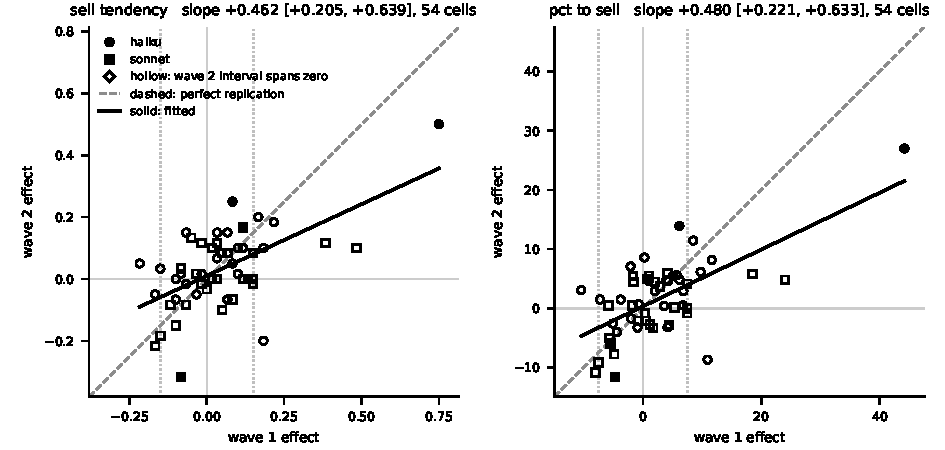
\includegraphics[width=\textwidth]{../figures/fig7_replication_acl.pdf}
  \caption{The 54 cells both waves carry, each plotted at its wave 1 effect
  against its wave 2 effect, on items the first wave never saw. If a
  wave 1 estimate were the truth, the cloud would sit on the dashed identity
  line; if the finding were noise, the cloud would be round. It is neither.
  It tilts, which is the replication, and it tilts at about half the identity
  slope, which is the shrinkage. Both axes carry the same range so that the
  identity line is drawn at forty five degrees and a reader can judge the gap
  by eye. The dotted verticals cut off the top quartile by wave 1 magnitude,
  the band that loses half of itself while the rest of the design does not
  move. A hollow marker is a cell whose wave 2 interval spans zero, which is
  most of them: this is a figure about where the points sit, not about which
  of them are significant.}
  \label{fig:replication}
\end{figure*}
\else
\begin{figure}[t]
  \centering
  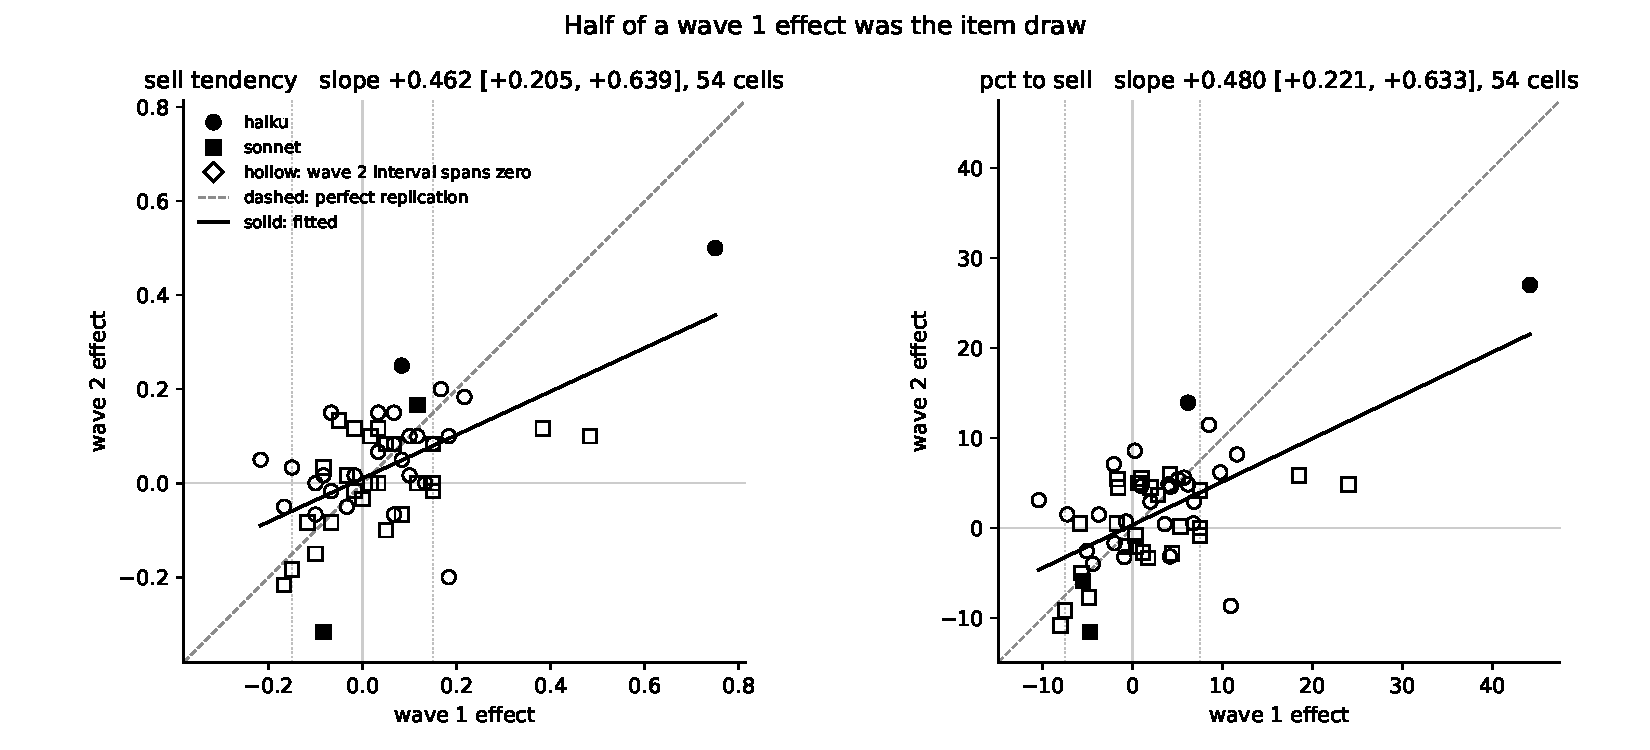
\includegraphics[width=\linewidth]{../figures/fig7_replication.pdf}
  \caption{Wave 2 against wave 1, one point per cell. The dashed line is
  perfect replication and the solid line is the fit. The gap between them is
  the regression to the mean, and the dotted verticals mark the top quartile
  by wave 1 magnitude, where all of it sits.}
  \label{fig:replication}
\end{figure}
\fi

\paragraph{The magnitudes do not replicate, and the reason is measurable.}
The disposition aggregate over the cells wave 2 covers is $+0.347$ $[+0.233,
+0.464]$ in wave 1 and $+0.147$ $[+0.014, +0.281]$ in wave 2; on the
continuous measure, $+18.375$ $[+12.542, +24.361]$ against $+7.728$
$[+0.881, +14.694]$. The between wave differences are $-0.200$ $[-0.375,
-0.022]$ and $-10.647$ $[-19.678, -1.611]$, intervals that exclude zero. Two
fifths of the wave 1 figure comes back. The obvious reading is that something
about the second wave is different, and it is the wrong one. Across all 54
cells, 28 came in smaller on the categorical measure and 26 on the
continuous one, against 27 under no attenuation whatsoever: there is no
general shrinkage to find. The shrinkage is conditional on size. The
correlation between a cell's wave 1 magnitude and the change in its magnitude
is $-0.580$ and $-0.622$, permutation $p$ 0.0001 on both measures. The top
quartile by wave 1 magnitude shrank in ten of thirteen cells, by $-0.117$ and
$-5.821$ on average, while the other three quartiles moved $+0.009$ and
$+0.631$, which is nothing.

\paragraph{One number for all of it.} Regressing each cell's wave 2 effect on
its wave 1 effect gives a slope of $+0.462$ $[+0.205, +0.639]$ on the
categorical measure and $+0.480$ $[+0.221, +0.633]$ on the continuous one,
resampled over cells rather than pairs. A slope of one is what wave 1
estimates being the truth would produce, and both intervals exclude it; a
slope of zero is what noise alone would produce, and both exclude that too.
The slope is therefore the fraction of a wave 1 effect that was signal rather
than a favourable item draw, measured on items the first wave never saw, and
it is a little under a half. Figure~\ref{fig:replication} is that fit, and
it is this section's argument in one picture: a cloud that tilts, at half the
slope it would tilt at if twelve pairs told the truth.

\paragraph{What that is.} Regression to the mean, measured from outside
rather than bounded from inside. A large effect at twelve pairs is partly a
large true effect and partly a favourable item draw, and only the first half
returns on items the first draw never saw. \movedref{sec:rtm} asks whether
the compression result is regression to the mean and can only bracket the
answer within one wave, because the sampling error it wants to subtract is
estimated from the same twelve pairs that carry the effect. A second draw
from the same generator is not subject to that circularity, and it puts a
number on the correction: the slope above, and in the quartile where this
paper's headline findings live, roughly half of a wave 1 magnitude is the
draw.

\paragraph{Both headline magnitudes attenuate, and both directions hold.}
The single cell this paper leads with, Haiku at \texttt{low} effort on the
disposition family, moves from $+0.750$ $[+0.483, +1.033]$ to $+0.500$
$[+0.167, +0.850]$ on the categorical measure and from $+44.167$ $[+28.500,
+60.333]$ to $+27.000$ $[+9.500, +46.333]$ on the continuous one, pooling to
$+0.625$ $[+0.400, +0.858]$ and $+35.583$ $[+22.958, +48.500]$, which still
survive Holm. The compression of the family spread behaves the same way:
Haiku's fall from \texttt{low} to \texttt{high} is $-0.085$ against wave 1's
$-0.160$ categorically and $-4.008$ against $-10.002$ continuously, and
Sonnet's continuous spread falls by $-0.039$ against $-3.499$ while its
categorical spread rises by $+0.020$ against a fall of $-0.070$. The spread
still falls in three of the four model by measure combinations wave 2 covers.
A reader who wants this paper's best estimate of either finding should take
the pooled figure and read the wave 1 figure as the upper end.

\paragraph{Two things the second wave cannot settle.} Opus is absent from it,
so the defect recorded in \movedref{app:disposition}, that Opus spans zero on
the disposition measures because its sign changes with effort, stands exactly
where wave 1 left it: the extension that would speak to it is the one the
budget did not reach. And the two measures are not two tests. They are two
readings of the same answer and they move together, so the attenuation is one
finding whose intervals exclude zero narrowly, not a pair of independent
confirmations.
